\documentclass[12pt]{article}
\usepackage{../template/NotesTeX}
\begin{document}
\setlength{\parskip}{\baselineskip}%
\graphicspath{ {/home/ab/school/notes/electeng101/} }

\title{Electeng101}
\author{Alexander Bailey}
\emailAdd{alexkingstonbailey@gmail.com}
\maketitle
\flushbottom

\section{Fundamentals of Electrical and Digital Systems}
\subsection{Electricity as Energy}
The fundamental concept that underpins the modern electrical `cycle' is: 
\begin{definition*}
  Energy is used to separate charges i.e the chemical reaction in a cell. This becomes the electric potential energy of the circuit
\end{definition*}

Separation of charge causes a difference in electric potential energy.
When this difference is applied to a closed circuit, charge will move around the circuit.
The movement of charge through is called a current. 

\subsubsection{Charge}
\begin{definition*}
  Electric charge is the physical property of matter that causes it to 

  experience a force when placed in an electromagnetic field. ($q$ or $Q$)
\end{definition*}

We (thanks to Benjamin Franklin) typically describe charge as having two states: postive (like a proton) and negative (like an electron).
These are not inherent to the universe but are just what we have defined.
Of course, the classic line is: `Like charges repel, opposite charges attract'.
Modeling the wire as a pipe carrying water, charge would be the amount of water. 

We model the strength of the electrostatic force as proportional to the charge of both particles and inversely proportional to the radius squared.
This is known as Coulomb's Law.

\begin{equation*}
  F \propto \frac{q_1q_2}{r^2}
\end{equation*}

Charge is measured in Coulombs (symbol C).
1C is is equivalent to approximately $6.3 \times 10^{18}$ electrons.

\subsubsection{Current}
\begin{definition*}
   Current is the rate of flow of charge represented by $i$ or $I$.
\end{definition*}

\marginnote{
  $I = {q\over t}$ \\
  or \\
  $I = \frac{dq}{dt}$
}[-1.1cm]

Current is defined numerically as the number of charges flowing through a particular point in one second.
Mathematically, it is the derivative of the total number of charges $q$ passing through a given section over time $t$ (written as $\frac{dq}{dt}$).
Current thusly has units of Coulombs per second ($\unit{Cs}^{-1}$) but Electrical Engineers have given this another name, the \textit{Ampere} (A).

\marginnote{Ampere also gave us the name current!}

Current gives Electrical Engineers an idea of how \textit{fast} energy is being used instead of how \textit{much} energy it has received\mn{Note that most electrical devices require a continuous supply of energy to function so speed is generally much more useful than amount }.
In the water analogy, current would be the speed of the water in the pipe. 

\begin{theorem*}
  \textbf{Conventional Current}

  Benjamin Franklin believed that electrical current was carried by positive charge `carriers', this led to \textit{centuries} of engineers using the wrong direction for current...
  Now we still use conventional current. BUT, electron flow is still in the other direction.
  Because of relative motion, a movement of negative charge in one direction is the \textbf{same thing} as a movement of positive charge in the other direction.
  Hence, it does not matter (for most things).
\end{theorem*}

\begin{theorem*}
  \textbf{Double-subscript notation}
  
  This notation indicates the directions charges are flowing in the order of \textbf{from} and \textbf{to}. 
  \begin{equation*}
    I_{ab} 
  \end{equation*}
  $I_{ab}$ is the current flowing from a to b.
\end{theorem*}

\begin{example}
  \begin{gather*}
    i = 0.5\unit{A } 
    t = 8\unit{min} = 60 \times 8 \unit{seconds} = 480\unit{seconds} \\
    i = \frac{dq}{dt} \\
    \implies q = \int_0^{480}0.5dt = [0.5t]_0^{480} \\
    \therefore q = 240\unit{C}
  \end{gather*}
\end{example}

\subsubsection{Voltage}
\begin{definition*}
  Voltage is the difference in electrical potential energy of each unit of charge between two points represented by $v$ or $V$.
\end{definition*}

Because a voltage is a difference, we must know what point in the circuit that the difference is measured relative to for it to make sense.
Voltage is commonly called a potential difference (PD) and has units Joules per Coulomb ($\unit{JC}^{-1}$).
Physically, it is the amount of energy lost or gained between two points. 
Using our water analogy, voltage would be the pressure of the water in the pipe.

Alessandro Volta decided that Joules per Coulomb ($\unit{JC}^{-1}$) was too difficult and gave us the \textit{Volt} (symbol V).
Additionally, every voltage must be accompanied by a \textit{voltage arrow}. 
This removes the ambiguity in which direction voltage is measured. 
The voltage arrow points in the direction of a \textit{potential rise}.

The voltage at A, with respect to B, is $V_{AB}$. 

\begin{theorem*}
  \textbf{Common Reference or Ground}

  Voltages are always measured between two points.
  It is convenient to define a reference where we can talk about voltages `at' a component.
  The location of ground is arbitrary and does not affect the actual voltages in the circuit.
  The `triangle' ground is for digital circuits while the `line' ground is for analog circuits.
\end{theorem*}
\begin{marginfigure}
  \vspace{ -1.8cm }
  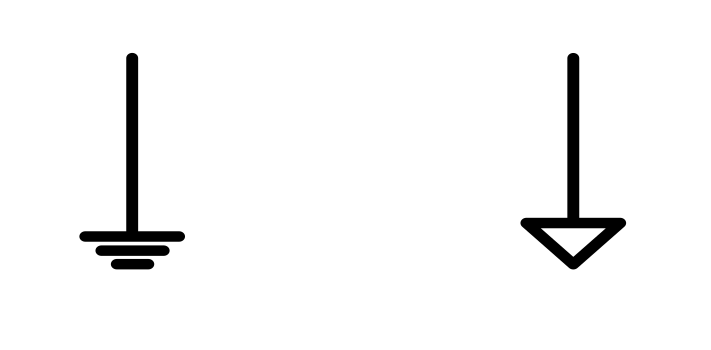
\includegraphics[scale=0.2]{grounds}
\end{marginfigure}


\begin{example}
  \begin{gather*}
    v = 2 - 6 \\
    v = iR \\
    -4 = 2i \\
    i = -2
  \end{gather*}
\end{example}
\begin{marginfigure}
  \vspace{ -1.5cm }
  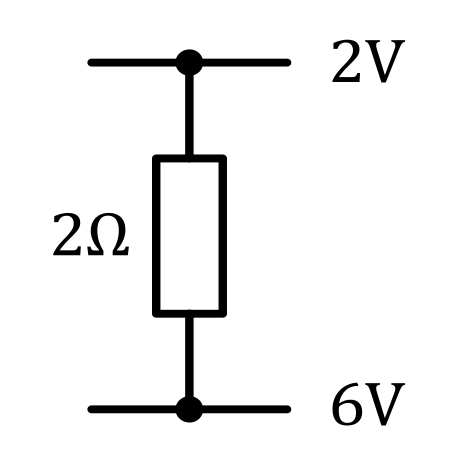
\includegraphics[scale=0.2]{example3}
\end{marginfigure}

\subsubsection{Resistance}

When electrical charge flows through a material, it must lose energy as it repels and collides with other charges.
The amount of energy lost depends on how `difficult' it is for the charge to flow. 
This difficulty depends on many factors including: stability of valence electrons, temperature, length and area.
These properties are summarised by \textit{resistance}.

\begin{equation*}
  v = i \times R 
\end{equation*}

\marginnote{Thinner materials have a higher resistance!}

From Ohm's Law, the amount of energy lost by the charges through a resistor is proportional to the rate at which charges slow through it.
The constant of proportionality $R$ from Ohm's Law is known as resistance. 
From this law, we can see resistance has units of Resistance has $\frac{V}{A}$.
We call this Ohms and give it the symbol Omega $(\Omega)$.

\begin{theorem*}
  \textbf{Conductance}

  Conductance is the inverse of resistance and has the symbol G. 
  It has units of \textit{Siemens} symbol $S$.
  It mostly exists so that you can add parallel conductances i.e for 2 2$S$ resistors in parallel, we have a conductance of 4$S$.
  With conductance, we would write Ohm's Law as $i=\nu G$.
\end{theorem*}

\begin{definition*}
  \textbf{The Passive-Sign Convention}

  When using Ohm's law there is an implicit sign convention that cannot be described by just the positive and negative symbols.
  A current is taken to be in the direction of a voltage drop. 
  This makes sense because charges can only lose energy through a resistor.
\end{definition*}

\begin{marginfigure}
  \vspace{-1cm}

  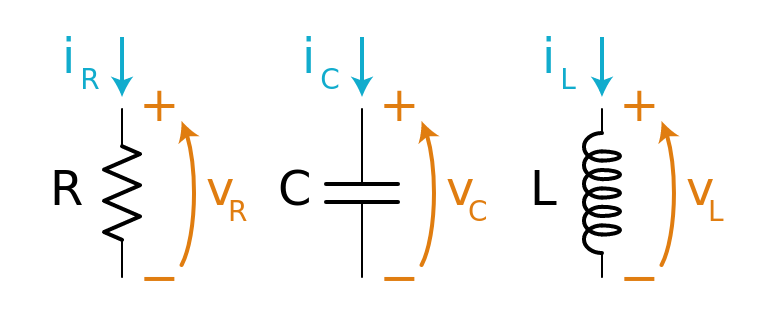
\includegraphics[scale=0.2]{convention}
\end{marginfigure}

\subsubsection{Power}
Power is the rate at which electric charges gain or lose electric potential energy.
Given that voltage is the difference in energy per $Q$ and current is the no. of $Q$ per sec, we can easily derive an equation for power:
\begin{multicols}{2}
\begin{equation*}
  P = IV 
\end{equation*}

\begin{equation*}
  P = \frac{dE}{dt} 
\end{equation*}
\end{multicols}
Dimensionally, this quantity would be measured in Js$^-1$ (Joules per Second).
This quantity is named the \textit{Watt} (symbol W) named after James Watt for his work with steam engines.

\marginnote{Watt is the unit of power?}

There is an assumed sign convention with power.
If V and I are in opposite directions then $p=vi$ otherwise $p=-vi$.
This is the passive-sign convention again.
Sticking to that, a negative power is power supplied.

\subsection{Circuit Definitions}
Here are some conventions used to describe all circuits:

\begin{tabular}{c|c}
load & `destination' of the electricity i.e. a lightbulb \\
topology & the nature of the connections between components \\
nodes & the point where two or more components meet \\
loop & a closed path starting and eventually returning to a node \\
\end{tabular}

When we are discussing values in a circuit, voltage is `across' a component, current is `through'. 
This means the voltage through a branch but we could also talk about the voltage `at' a component.
`at' means the PD is measured from the point to ground.

\begin{theorem*}
{\bf Circuit Topologies}
\begin{center}
\textbf{Closed}
\end{center}
The circuit has both flow of charge and energy transfer.

\begin{center}
\textbf{Open}
\end{center}

No electric potential means no flow of charge and no energy transfer. 
The circuit could be disrupted, i.e there is an air gap with (theoretically) infinite resistance.

\begin{center}
\textbf{Short}
\end{center}

The circuit (or circuit section) has a 0v potential difference.
This could mean a path of lower resistance meant no voltage `went' down that path or that voltages cancelled etc.
\end{theorem*}

\subsection{Components}

\subsubsection{Ideal Wire}
Ideal Wire has a resistance of 0$\Omega$. 
This means that no energy is lost when a current goes through it. 
This is obviously useful as a model for electrical engineering but causes problems with some cases.
For example, connecting an ideal wire across the terminal of a voltage source creates a theoretically \textit{infinite} amount of energy.

\subsubsection{Voltage and Current Sources}
These sources can receive or output an \textit{infinite} amount of energy without deviating from their specification.
These are good models in most well-designed engineering applications because the sources are designed to operate within their limits.

Ideal Voltage Sources maintain a constant voltage across its terminals.
This means it will draw (or supply) whatever current is necessary to maintain that voltage.
Meaning the current is dependent on the topology of the circuit.
Don't connect them in parallel.

Ideal Current sources don't actually exist.
But they maintain a constant current through its terminals regardless of voltage. 
This behaviour means that the voltage across it depends on the topology of the circuit.

\subsection{Tools}
There are a number of mathematical tools that we have developed to make solving circuits easier.

\subsubsection{KCL}
Kirchoff's Current Law describes the behaviour of current in a circuit, it is:
\begin{theorem*}
  The algebraic sum of the currents leaving any point in a circuit equals zero.
\end{theorem*}
This means the amount of charge arriving at any point in one second \textbf{must} equal the amount of charge leaving that point in one second.
Therefore,
\begin{equation*}
  \sum I_{in} = \sum I_{out}
\end{equation*}

If we don't know the current direction, just make them all leaving and it the maths will show us if a current is entering because it will be negative.
The general process is hence:

\begin{enumerate}
  \item Assign current directions 
  \item Assign directions for voltages 
  \item Form an equation in terms of $i_n$
  \item Substitute unknowns for knowns using Ohm's Law 
\end{enumerate}

\subsubsection{KVL}
Kirchoff's Voltage Law describes the behaviour of voltages in a circuit, it is:
By the conservation of energy, energy gained in a circuit equals the energy lost.
Therefore, the total voltage rises must equal the total voltage drops. Hence,

\begin{theorem*}
  The algebraic sum of the voltage rises around a loop in a circuit equals zero
\end{theorem*}

Once again, if we assume a direction we can solve for the unknown directions.
The process for KVL is generally:

\begin{enumerate}
  \item Assign voltage polarities 
  \item Identify Loops
  \item Form equations (taking voltage rises as positive)
\end{enumerate}
\begin{example}
  \begin{align*}
    &\text{Assign Voltage Polarities,}\\
    &\text{Loop 1: } 5-(2I_1)-(-4I_2)-3=0 \\
    &\text{Loop 2: } 3-(4I_2)-(-6I_3)=0 \\
    &\text{Loop 3: } 5-(2I_1)-(-6I_3)=0 \\
    &\text{Then you can solve simultaneously using KCL} \\
    &\text{KCL: }-I_1 -I_2 = I_3 \\
  \end{align*}
\end{example}
\begin{marginfigure}
  \vspace{-5cm}
  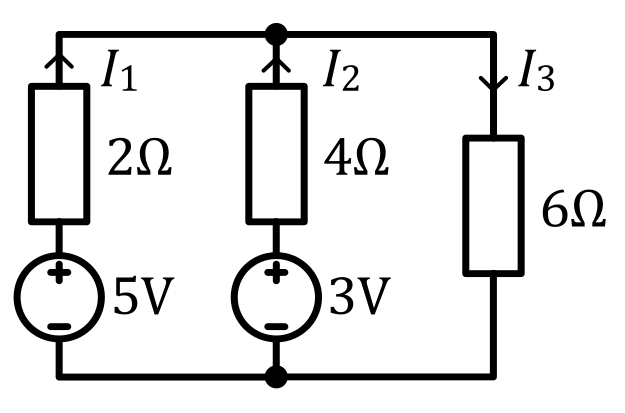
\includegraphics[scale=0.2]{kvl}
\end{marginfigure}

\subsubsection{Terminal Behaviour}
To analyse a circuit (determine current and voltage through every component), we need Kirchoff's laws and the \textit{terminal behaviour} of the components.
From these, useful shortcuts and `tricks' have been developed.

\subsubsection{Equivalent Resistance}
Equivalent Resistance is a way of helping us model the behaviour of a circuit as a resistor.
This is a simplification we can make, modelling a load as a static resistor value (no matter what the load actually is).
We can do this because from the source's `perspective', it cannot tell the load apart from this fixed resistance.
\marginnote{Series means there is only one path for the charges to flow through them (connected end-to-end)}

In Series
\begin{equation*}
  r = r_1 + r_2 + \dots + r_n = \sum^N_{k=1} r_k
\end{equation*}
In Parallel
\begin{equation*}
  r = \frac{1}{\frac{1}{r_1} + \frac{1}{r_2} + \dots + \frac{1}{r_n}} = \frac{1}{\sum^N_{k=1}\frac{1}{r_k}}
\end{equation*}

\marginnote{Parallel components have both of their ends connected together}

In series, r is always larger than any one of the components.
In parallel, r is smaller than the smallest resistor contributing to the resistance. 

We can use a systematic method to simplify compound circuits i.e.
\begin{enumerate}
  \item Begin as far away as possible from the source or component
  \item Replace series or parallel resistors with equivalent resistors
  \item Continue moving left and simplifying until we are left with only one
\end{enumerate}

\subsubsection{Voltage and Current Division}
Voltage Division is an easy way to find the voltage over resistors in series.
A voltage \textit{divider} is two (or more) resistors in series so $v_{\text{in}}$ is related to $v_{\text{out}}$ by a ratio dependent on the resistance.

So for two resistors, where $v_1$ is the voltage drop on the first resistor and $v_2$ is the voltage drop on the second resistor:
\begin{align*}
  v_1 = (\frac{R_1}{R_1 + R_2})V_s \\
  v_2 = (\frac{R_2}{R_1 + R_2})V_s \\
\end{align*} 

So for N resistors:
\begin{align*}
  v_p = (\frac{R_p}{R_1 + R_2 + \dots + R_p})V_s \\
\end{align*} 

\begin{marginfigure}
  \vspace{-10cm}

  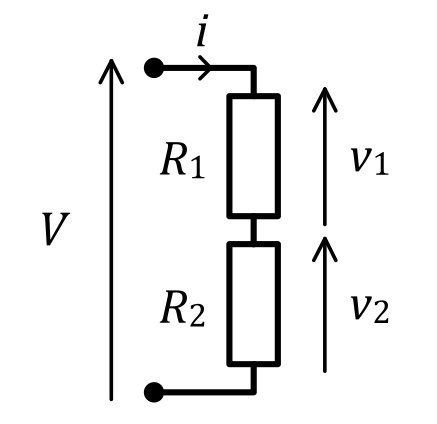
\includegraphics[scale=0.3]{voltagedivider}
\end{marginfigure}

Current Division is an easy way to find the \textit{current} over resistors in parallel.
Current in a current divider is related to a very similar ratio.

So for N resistors:
\begin{align*}
  v_p = (\frac{\frac{1}{R_p}}{\frac{1}{R_1} + \frac{1}{R_2} + \dots + \frac{1}{R_p}})I \\
\end{align*} 

\begin{marginfigure}
  \vspace{-5cm}

  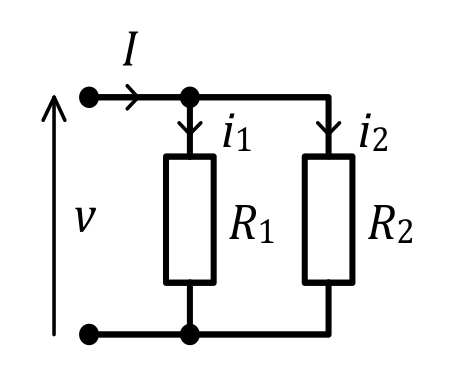
\includegraphics[scale=0.3]{currentdivider}
\end{marginfigure}

\subsubsection{Node-Voltage Analysis}
Not all circuits can be simplified into series or parallel resistors.
This brought around the need for node-voltage analysis.
We of course could apply KCL and KVL to solve these circuits but these methods require some adhoc/non-systematic thinking.

Node-voltage analysis is the use of KCL to find the voltages at nodes by expressing the currents through these nodes in terms of their voltages. 

Essential nodes are nodes that are connected to \textit{three} or more paths. 

\begin{enumerate}
  \item Select one of the essential nodes as the reference (ground) node, in which all other node voltages will be calculated with respect to.
  \item Write a KCL equation for each of the remaining essential nodes in terms of the unknown essential node voltages.
  \item Solve the node-voltage equations simultaneously.
\end{enumerate}

\begin{example}

\end{example}

\subsubsection{Superposition}
Superposition is the `divide and conquer' of EE. 
The Superposition Theorem states that: Any \textit{linear} response in a circuit containing multiple sources is equal to the algrebraic sum of the contributions to that response.
A linear response means that you can only calculate current and voltage \textbf{NOT} power.
However, you can separately calculate voltage and current and then calculate power. 
The steps are as follows:

\begin{enumerate}
  \item Set all but one of your current and/or voltage supplies to zero
  \item Solve this circuit for the desired values 
  \item Do this for each of your sources
  \item Sum each of your results i.e $i_1=i_{1(a)}+i_{1(b)}$
\end{enumerate}
\marginnote{Setting these to zero means different things! For a voltage supply, it becomes an ideal wire but a current source becomes a gap in the wiring!}[-3cm]

\begin{example}

\end{example}

\subsubsection{Th\'enevin's Theorem}
This theorem from french physicist Léon Charles Thévenin allows you to simplify \textit{any} collection of sources, wire and resistors into just one voltage source and one resistor (and the load).
\begin{enumerate}
  \item Remove the load you want to base the circuit around
  \item Calculate the Th\'enevin voltage ($V_{TH}$) by calculating the voltage over the gap where the load was
  \item Calculate the Th\'enevin resistance ($R_{TH}$) by pretending to be a current starting at one end in the gap where the load was and going to the other end, the resistances you pass through add to become the $R_{TH}$
  \item Put it all together. A voltage source that outputs $V_{TH}$ in series with a resistor $R_{TH}$, in series with the load.
\end{enumerate}

\begin{example}

\end{example}


\subsection{Models}
In Electrical Engineering (EE), a model is a description that communicates

\begin{itemize}
  \item Physical Characteristics 
  \item Electrical Function
  \item Magnitude
\end{itemize}

\marginnote{
Some EE models include:

\begin{itemize}
  \item Component Symbols 
  \item Schematics
  \item Block Diagrams 
  \item PCB Layouts 
\end{itemize}
}[-1cm]

\vspace{3pt}
Models allow you to more easily handle complex systems.
They compartmentalise systems into smaller sub-systems.
In circuit diagrams, component symbols are models of the actual components.
We can then focus on our actual engineering instead of {\it why} we are doing what we are doing (leave that to the physicists).

Mathematical Models, such as Ohm's Law, are still models. 
They simplify our calculations by making an approximation.

\section{SMART Engineering}
\begin{definition*}
  Systems of Monitoring, Analysis, and Response Technologies
\end{definition*}

\section{Electricity Supply}

\end{document}
